\section{Results}
\subsection{Temperature input}
Monthly mean T2M follows the same seasonal cycle at all three sites, from about \Tmin$^\circ$C in January to \Tmax$^\circ$C in April 2024 (\cref{fig:temp}). Mean battery temperature is \TcKhulna, \TcChuadanga{} and \TcRajshahi$^\circ$C at Khulna, Chuadanga and Rajshahi, a spread of \Tspread$^\circ$C (\cref{tab:results}).
\begin{figure}[t]\centering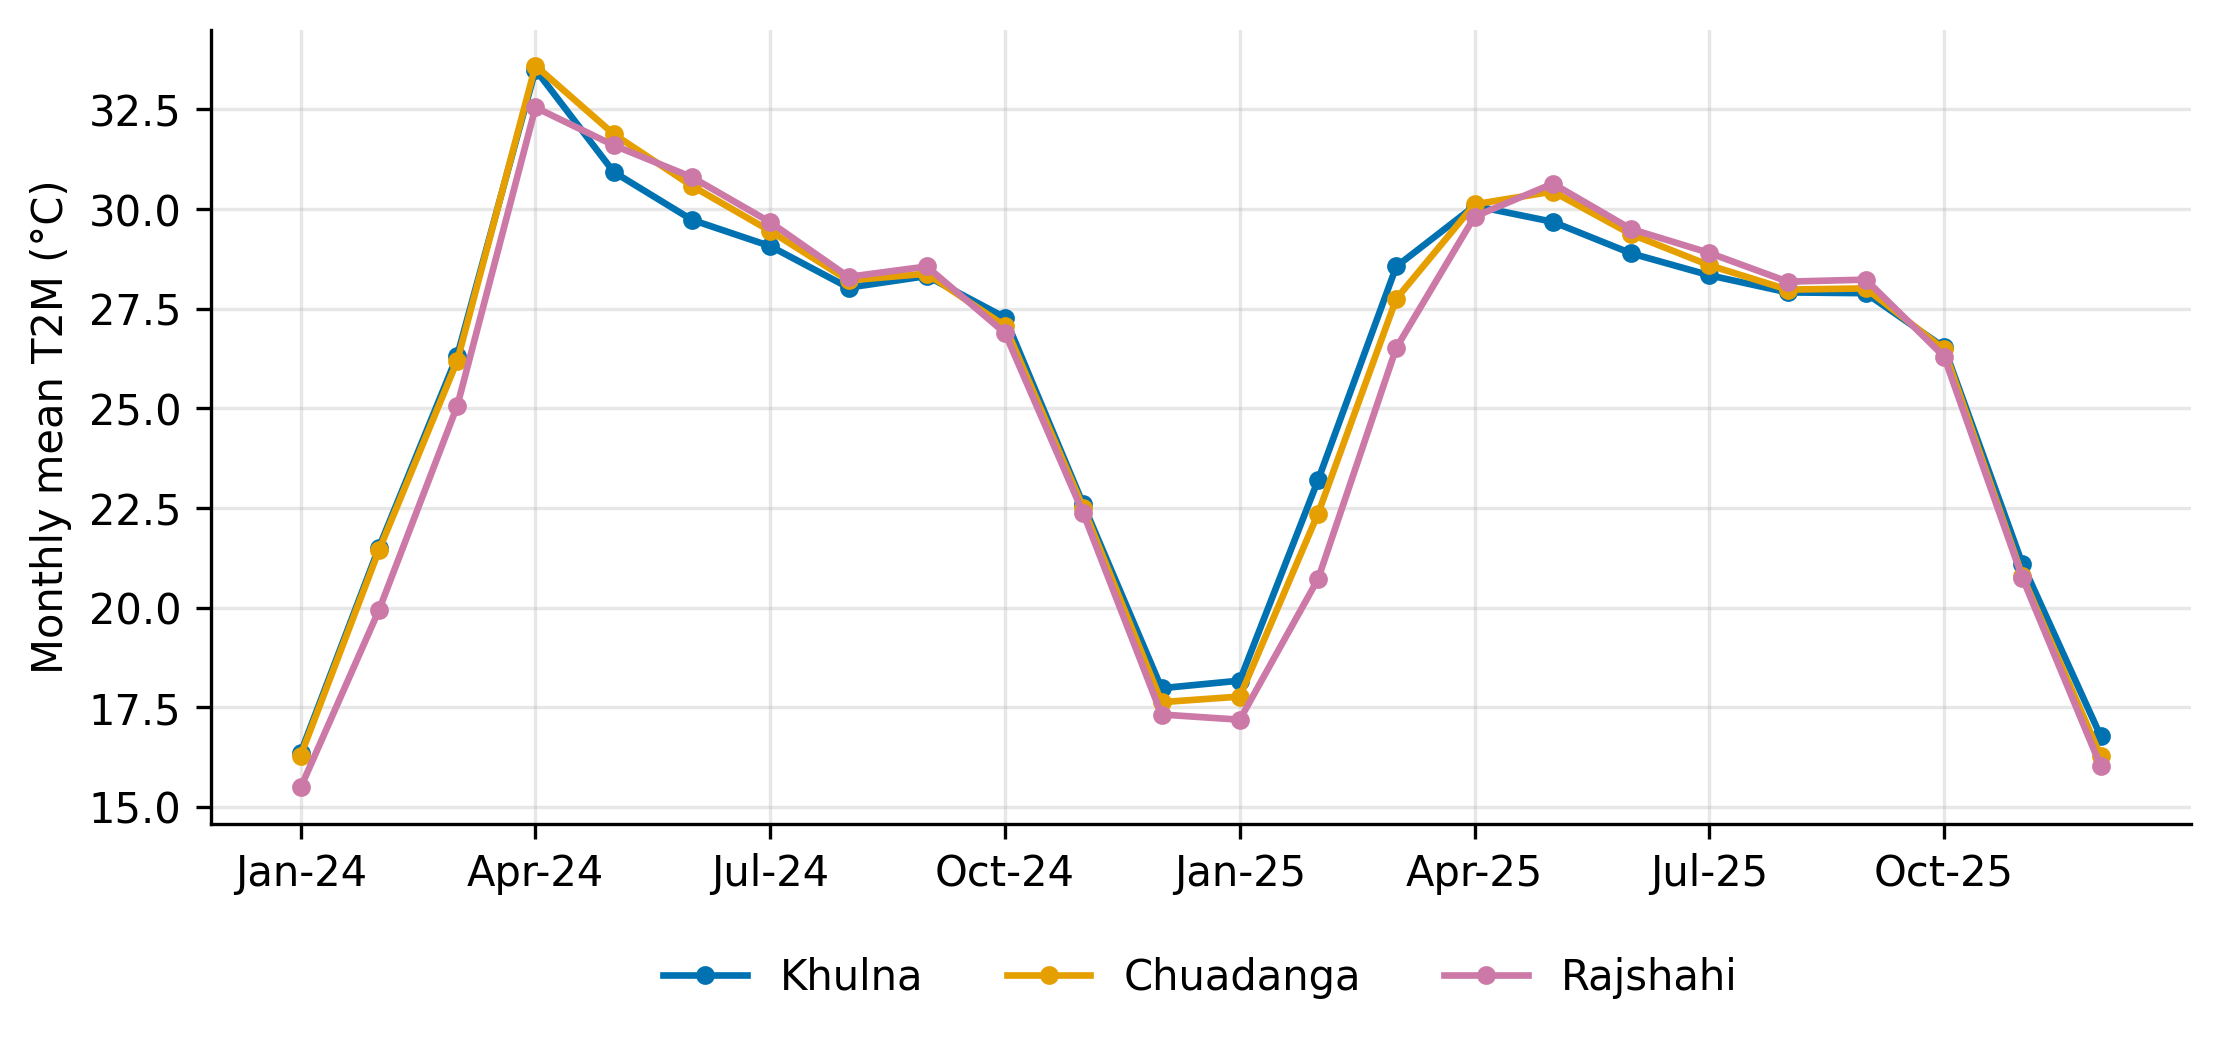
\includegraphics[width=.8\textwidth]{fig1_temperature.png}\caption{NASA POWER monthly mean 2\,m temperature at the three sites, Jan 2024--Dec 2025.}\label{fig:temp}\end{figure}

\subsection{Performance, life and cost}
\begin{table*}[t]
\centering\small
\caption{Simulated 24-month results (NASA POWER monthly $T_{2m}$, Jan 2024--Dec 2025; battery temperature = ambient + 5~$^\circ$C). Source: \texttt{results\_summary.csv} from \texttt{easybike\_main.m}. Life is in months of operation at 300~days\,yr$^{-1}$; TCO is net present value at an 11.57\% discount rate and a tariff of BDT 11.36/kWh.}
\label{tab:results}
\begin{tabular}{llrrrrrrrrr}
\toprule
Site & Battery & $\bar T_{cell}$ & $\eta$ & DoD & Range & $E_{grid}$ & Life & Repl. & TCO$_{10}$ & Cost \\
 & & ($^\circ$C) & (\%) & (\%) & (km) & (kWh/d) & (mo) & (10~yr) & ($10^3$ BDT) & (BDT/km) \\
\midrule
Khulna & Lead-Acid & 30.8 & 90.2 & 63.5 & 83.3 & 8.10 & 12.4 & 9 & 725 & 6.37 \\
 & LFP & 30.8 & 97.8 & 69.4 & 76.1 & 6.87 & 83.7 & 1 & 342 & 3.00 \\
 & NMC & 30.8 & 96.7 & 69.5 & 76.0 & 7.03 & 52.9 & 2 & 437 & 3.84 \\
\midrule
Chuadanga & Lead-Acid & 30.8 & 90.2 & 63.5 & 83.3 & 8.10 & 12.2 & 9 & 731 & 6.42 \\
 & LFP & 30.8 & 97.8 & 69.4 & 76.1 & 6.87 & 83.2 & 1 & 342 & 3.01 \\
 & NMC & 30.8 & 96.7 & 69.5 & 76.0 & 7.03 & 52.8 & 2 & 437 & 3.84 \\
\midrule
Rajshahi & Lead-Acid & 30.5 & 90.0 & 63.7 & 83.0 & 8.13 & 12.4 & 9 & 724 & 6.36 \\
 & LFP & 30.5 & 97.8 & 69.5 & 76.0 & 6.88 & 84.0 & 1 & 341 & 2.99 \\
 & NMC & 30.5 & 96.7 & 69.6 & 75.9 & 7.04 & 52.9 & 2 & 437 & 3.84 \\
\bottomrule
\end{tabular}
\end{table*}

\Cref{tab:results,fig:comp} give the main comparison. Discharge efficiency is about \effLA\% (LA), \effLFP\% (LFP) and \effNMC\% (NMC). Modelled life is \lifeLA{} months for LA, \lifeNMC{} for NMC and \lifeLFP{} for LFP (site mean), i.e.\ about \repLA{} LA packs but \repLFP{} LFP pack replacement in ten years. The 10-year net present cost per bike is BDT \tcoLA{} (LA), \tcoNMC{} (NMC) and \tcoLFP{} (LFP): LFP saves BDT \tcoSave{} per bike, and its cost per km (\cpkLFP\ BDT) is less than half that of LA (\cpkLA\ BDT). The LA bank has the longest range (\rngLA{} vs \rngLFP~km) because it stores more energy (9.0 vs 7.7~kWh), not because it is more efficient. All packs run close to the 80\% DoD limit in some months (maximum \dodmaxLA/\dodmaxLFP/\dodmaxNMC\%), which is realistic for easy-bike duty.
\begin{figure}[t]\centering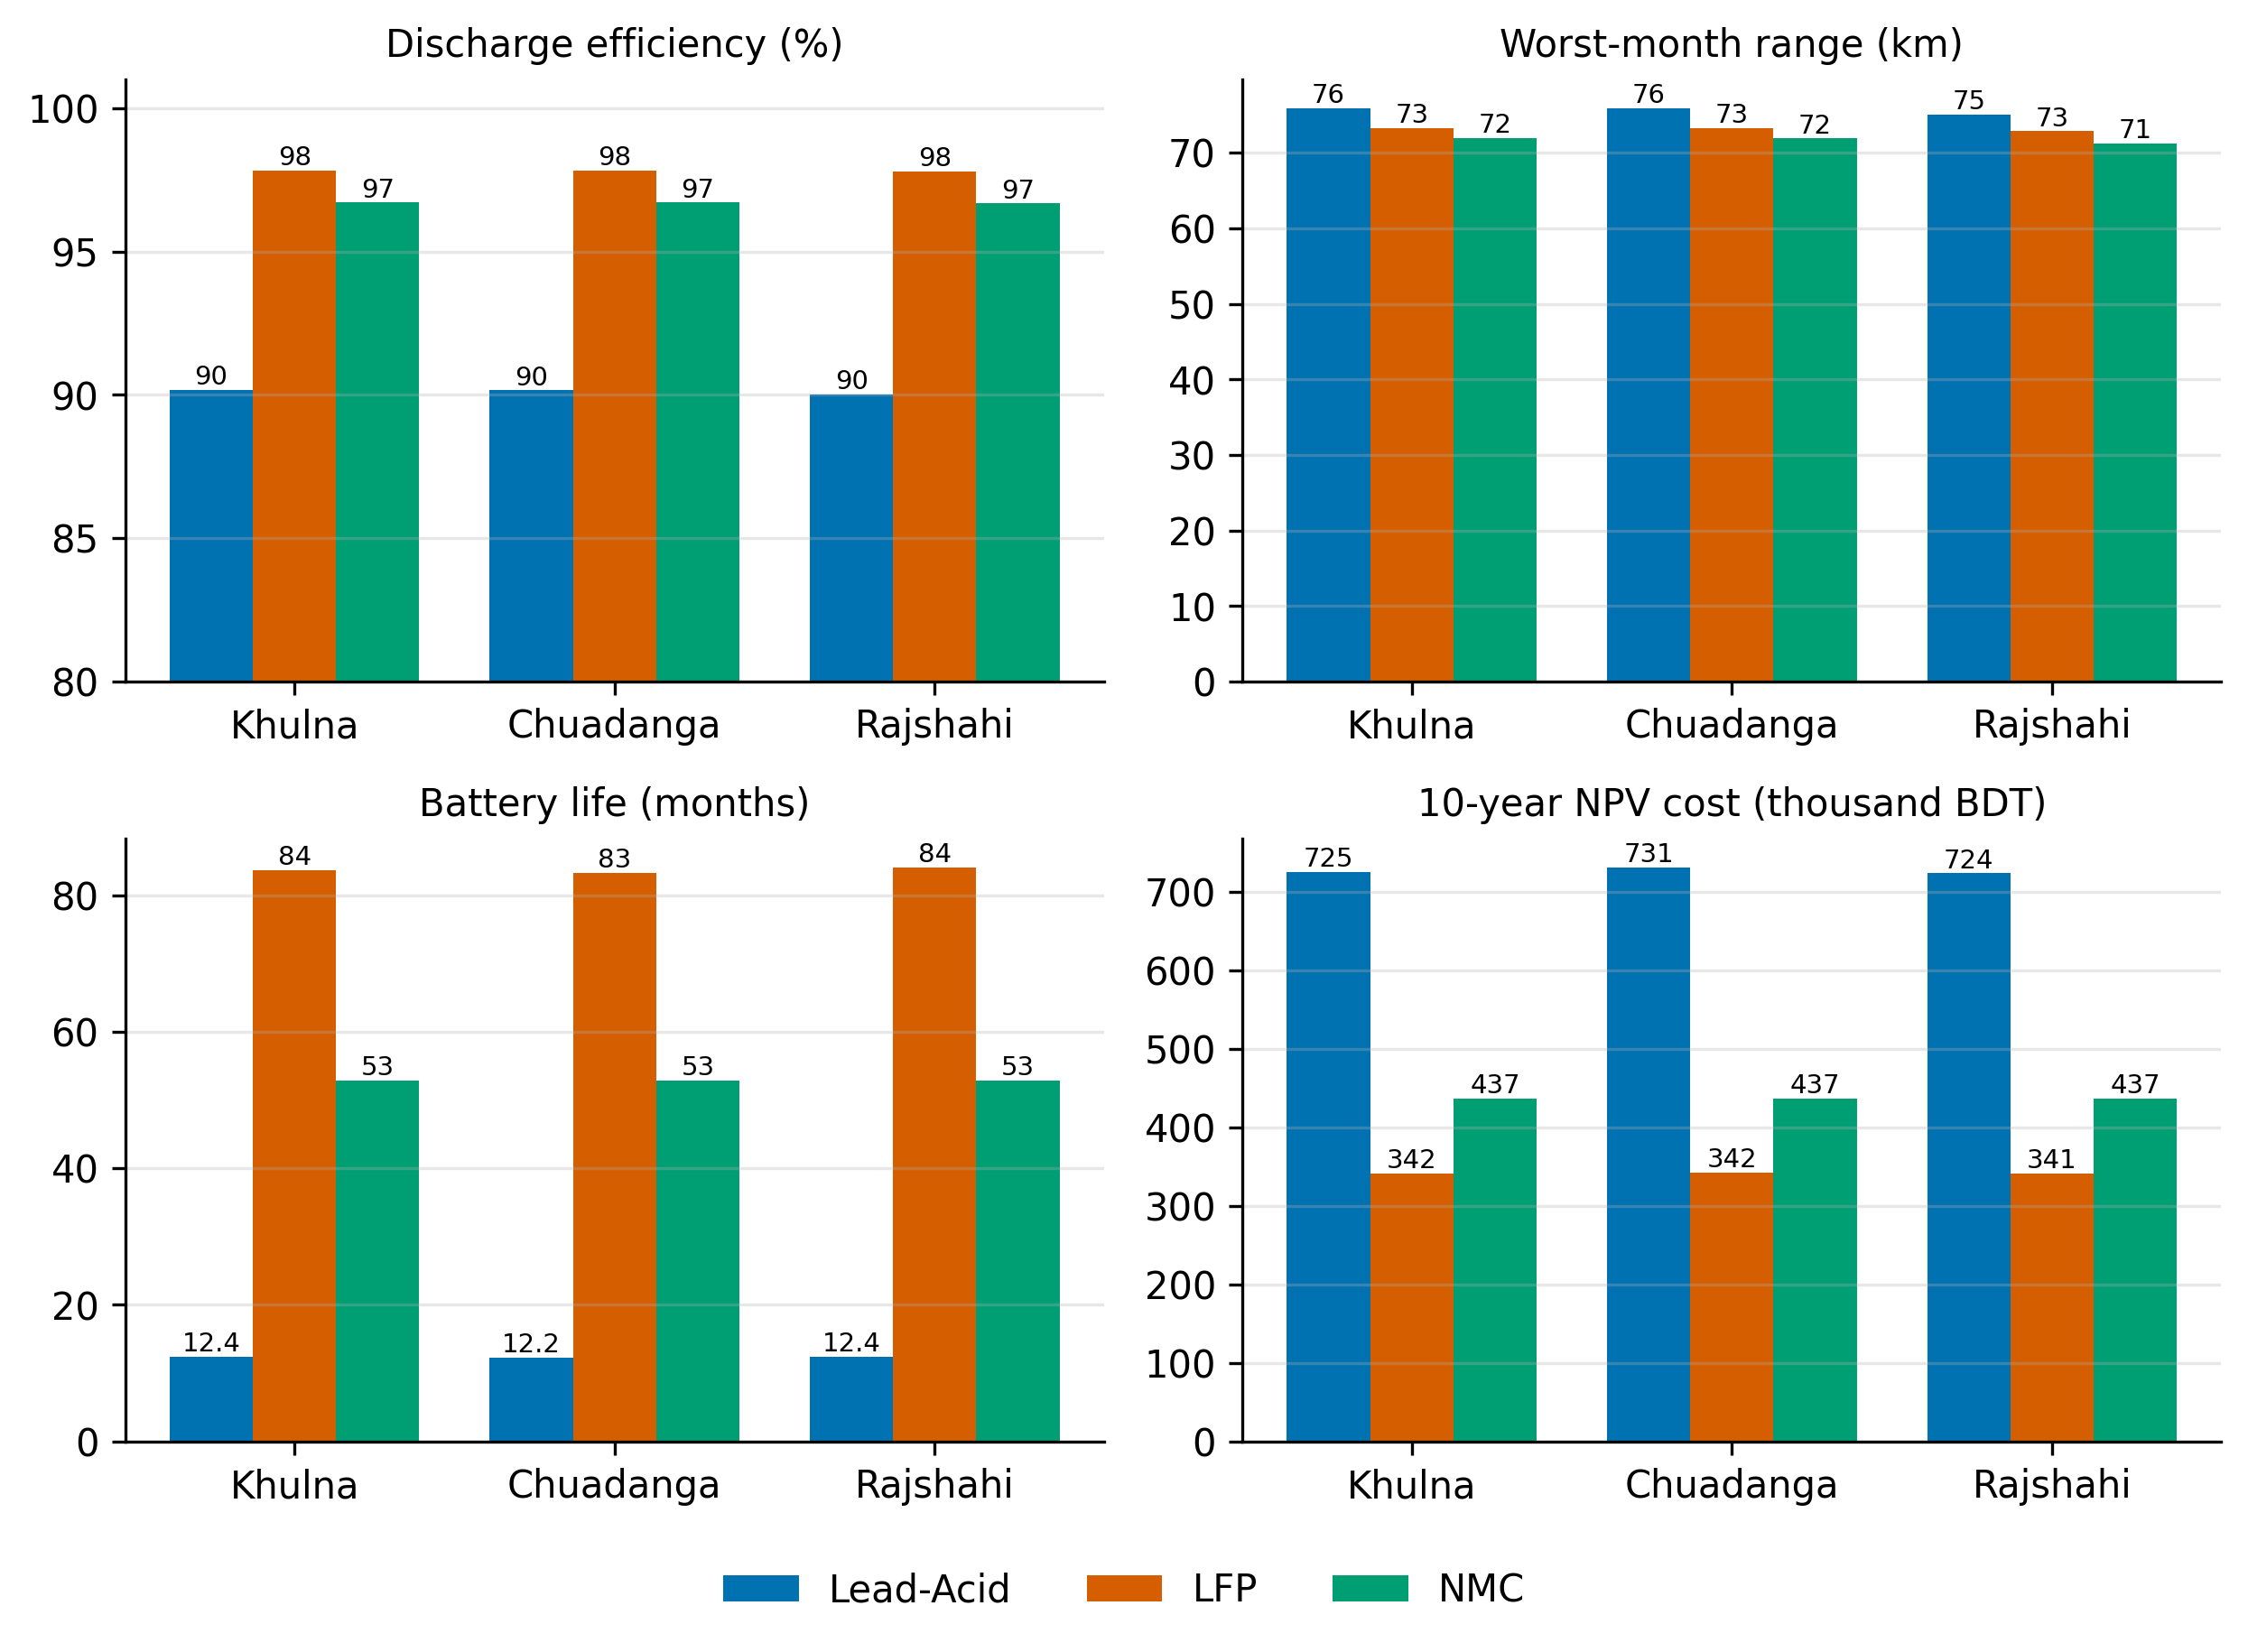
\includegraphics[width=.9\textwidth]{fig2_comparison.png}\caption{Site comparison of discharge efficiency, worst-month range, battery life and 10-year NPV cost.}\label{fig:comp}\end{figure}
\begin{figure}[t]\centering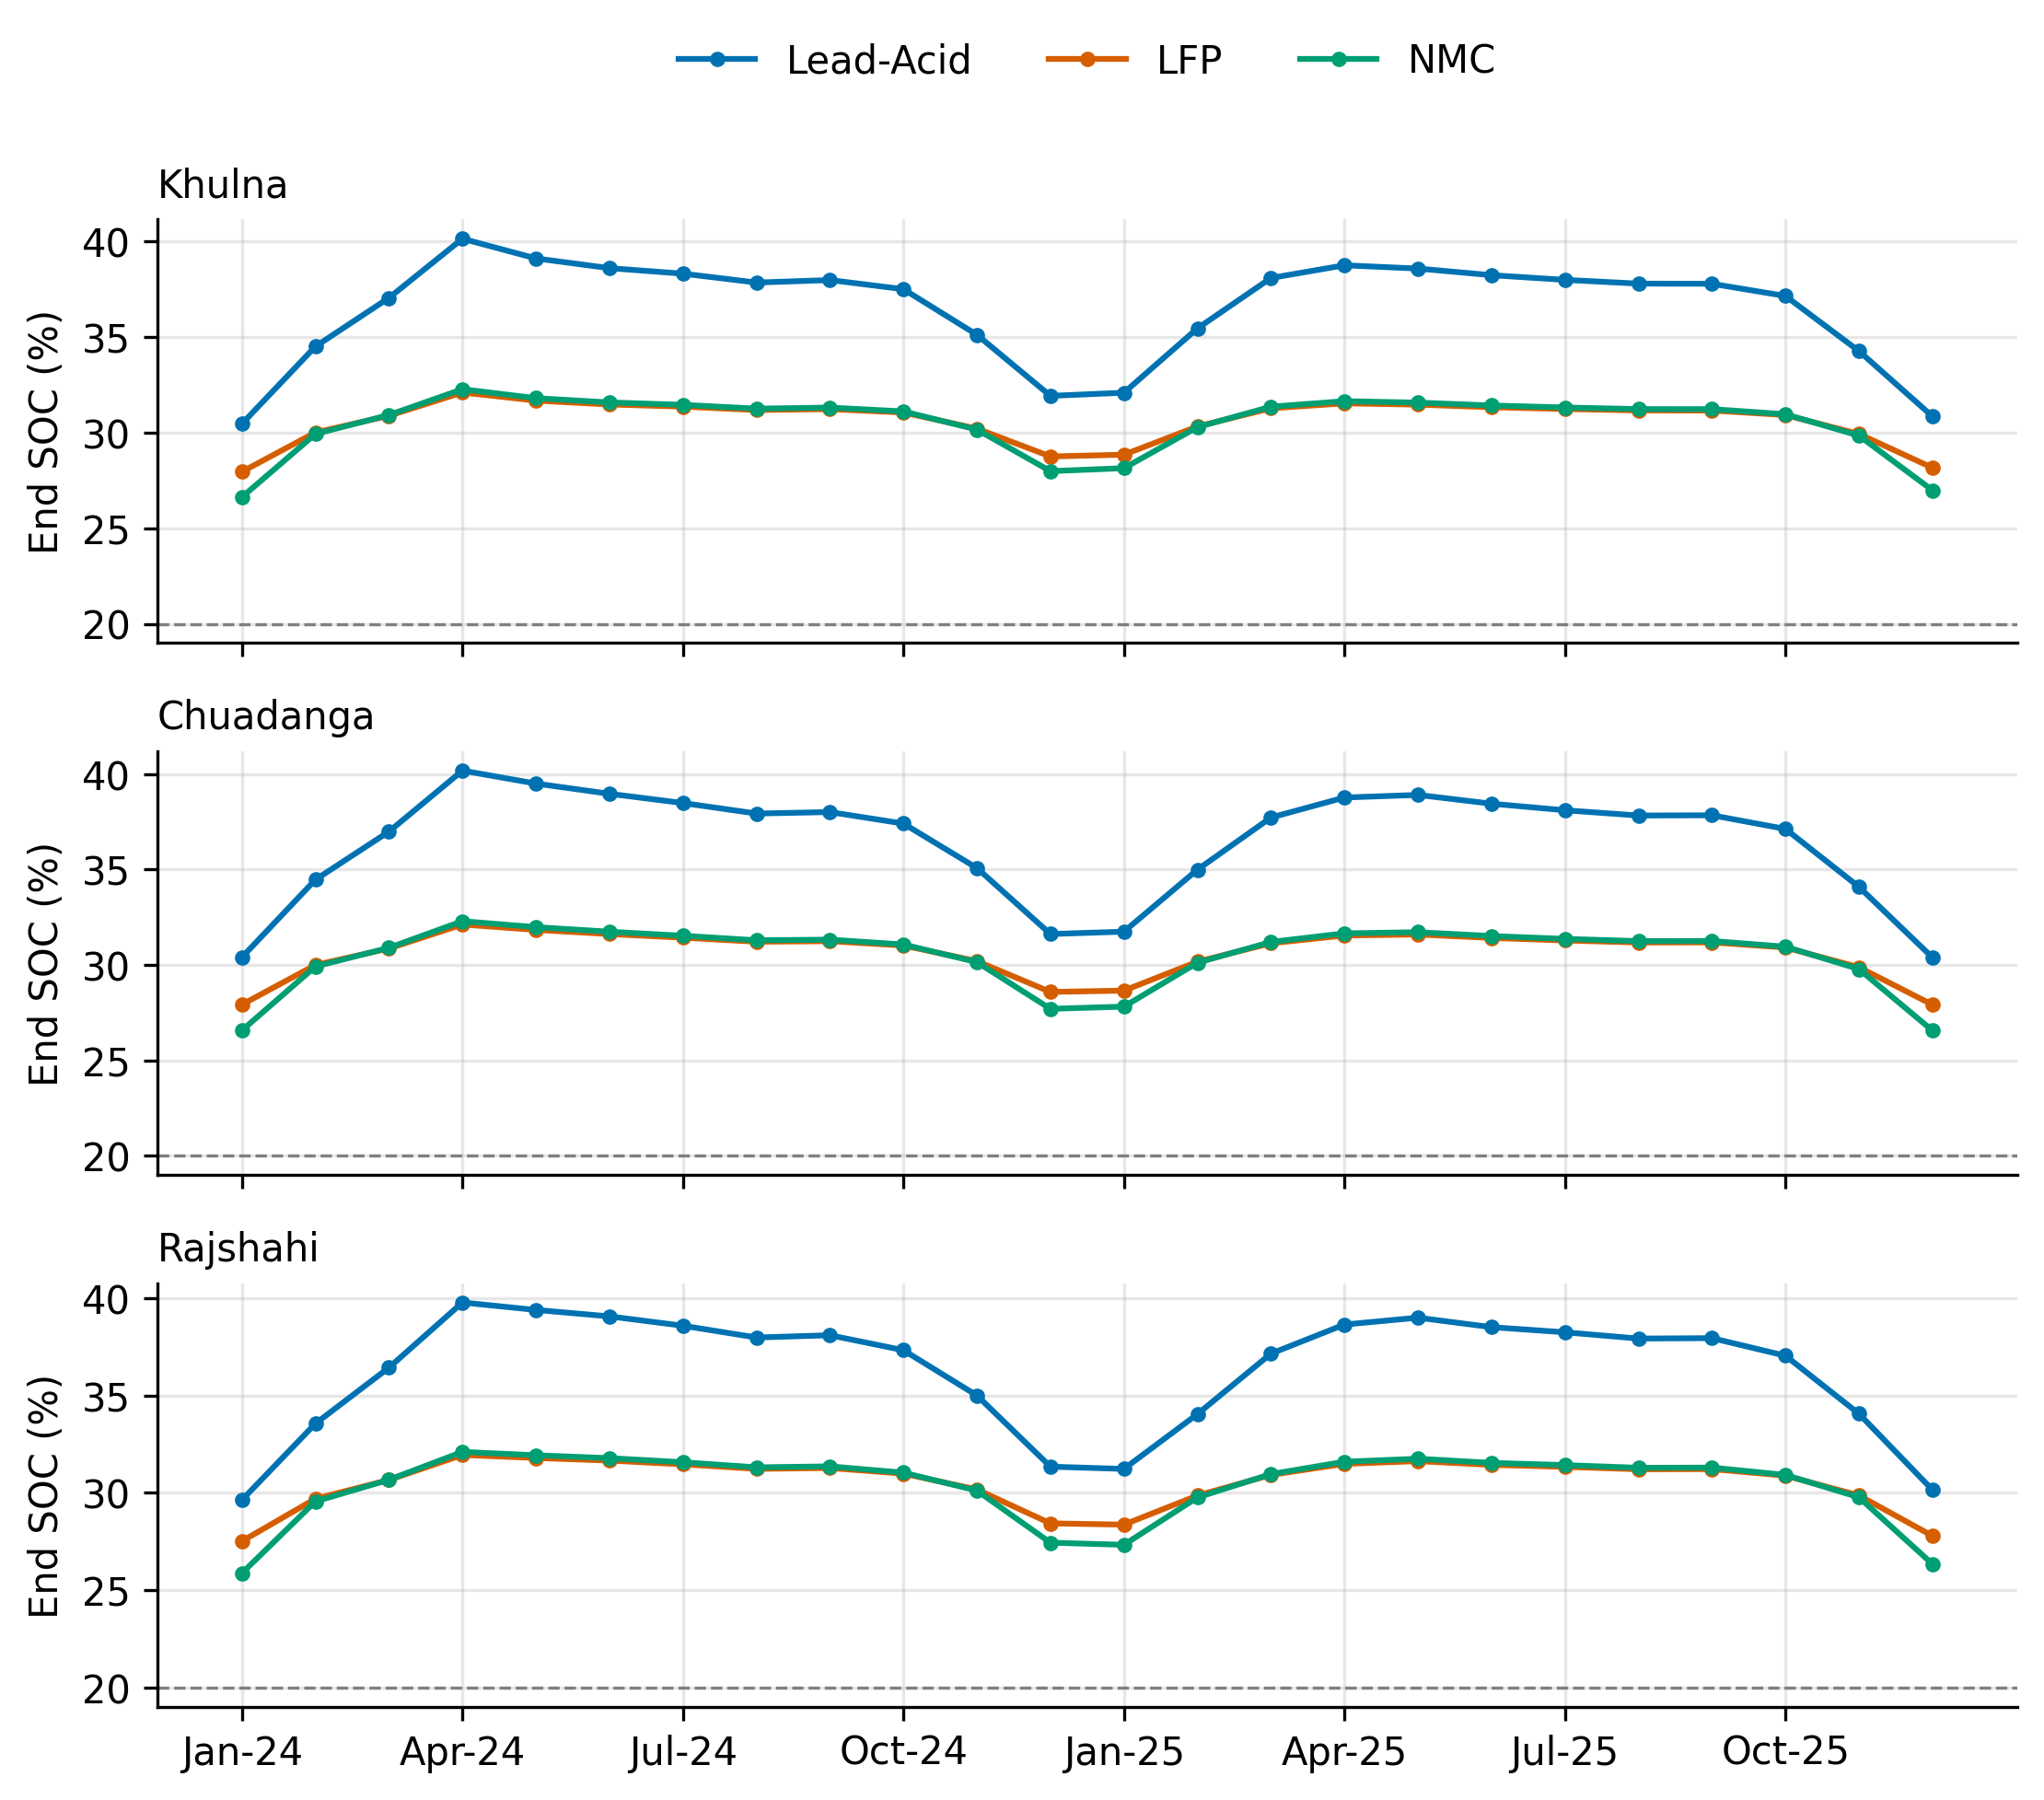
\includegraphics[width=.85\textwidth]{fig3_soc.png}\caption{Month-end state of charge after one day's discharge; dashed line = 20\% limit.}\label{fig:soc}\end{figure}

\subsection{Heat-wave stress}
At 42$^\circ$C ambient (Chuadanga, 10 May 2025 \citep{heat2025}) with the 5$^\circ$C offset, LA ages \heatLA{} times, LFP \heatLFP{} times and NMC \heatNMC{} times faster than in the 2024--25 monthly-mean climate. The absolute life gap between lead-acid and lithium therefore widens in heat.

\subsection{Scenarios, sensitivity and break-even}\label{sec:sens}
\begin{table}[t]
\centering\small
\caption{Scenario runs for inputs without a published source. Upper block: battery temperature rise above ambient (site mean). Lower block: daily distance at Chuadanga (max DoD $>$100\% means the pack cannot serve the duty).}
\label{tab:scen}
\begin{tabular}{lrrrrrr}
\toprule
 & \multicolumn{3}{c}{Life (months)} & \multicolumn{3}{c}{10-yr TCO (10$^3$ BDT)} \\
 & LA & LFP & NMC & LA & LFP & NMC \\
\midrule
$\Delta T$ = +0 $^\circ$C & 16.3 & 98.9 & 54.0 & 604 & 321 & 433 \\
$\Delta T$ = +5 $^\circ$C & 12.4 & 83.6 & 52.9 & 727 & 342 & 437 \\
$\Delta T$ = +10 $^\circ$C & 8.7 & 68.1 & 50.7 & 950 & 370 & 446 \\
\midrule
40 km/day (max DoD 42/44/45\%) & 24.7 & 137.3 & 87.1 & 397 & 237 & 295 \\
60 km/day (max DoD 63/66/67\%) & 14.0 & 91.5 & 58.1 & 649 & 317 & 402 \\
66 km/day (max DoD 70/72/73\%) & 12.2 & 83.2 & 52.8 & 731 & 342 & 437 \\
80 km/day (max DoD 84/87/89\%) & 9.4 & 68.7 & 43.6 & 932 & 398 & 515 \\
100 km/day (max DoD 105/109/111\%) & 6.8 & 54.9 & 34.9 & 1240 & 480 & 627 \\
\bottomrule
\end{tabular}
\end{table}

\Cref{tab:scen} shows that the battery temperature rise and daily distance change life and cost strongly. A battery 10$^\circ$C above ambient cuts LA life to 8.7 months, while 0$^\circ$C raises it to 16.3. At 100~km per day none of the three packs can serve the duty within 100\% DoD, and at 40~km per day all last far longer. The tornado chart (\cref{fig:tornado}) ranks daily distance, battery temperature rise and energy use above price, tariff or ageing parameters. LFP stays cheaper than LA up to an LFP pack price of BDT \beLFP{} (model price \priceLFP), BDT \beDistLow{} at 40~km per day and BDT \beTten{} at +10$^\circ$C. The up-front premium of BDT \premium{} is repaid in about \paybackYr{} year of running savings (undiscounted).
\begin{figure}[t]\centering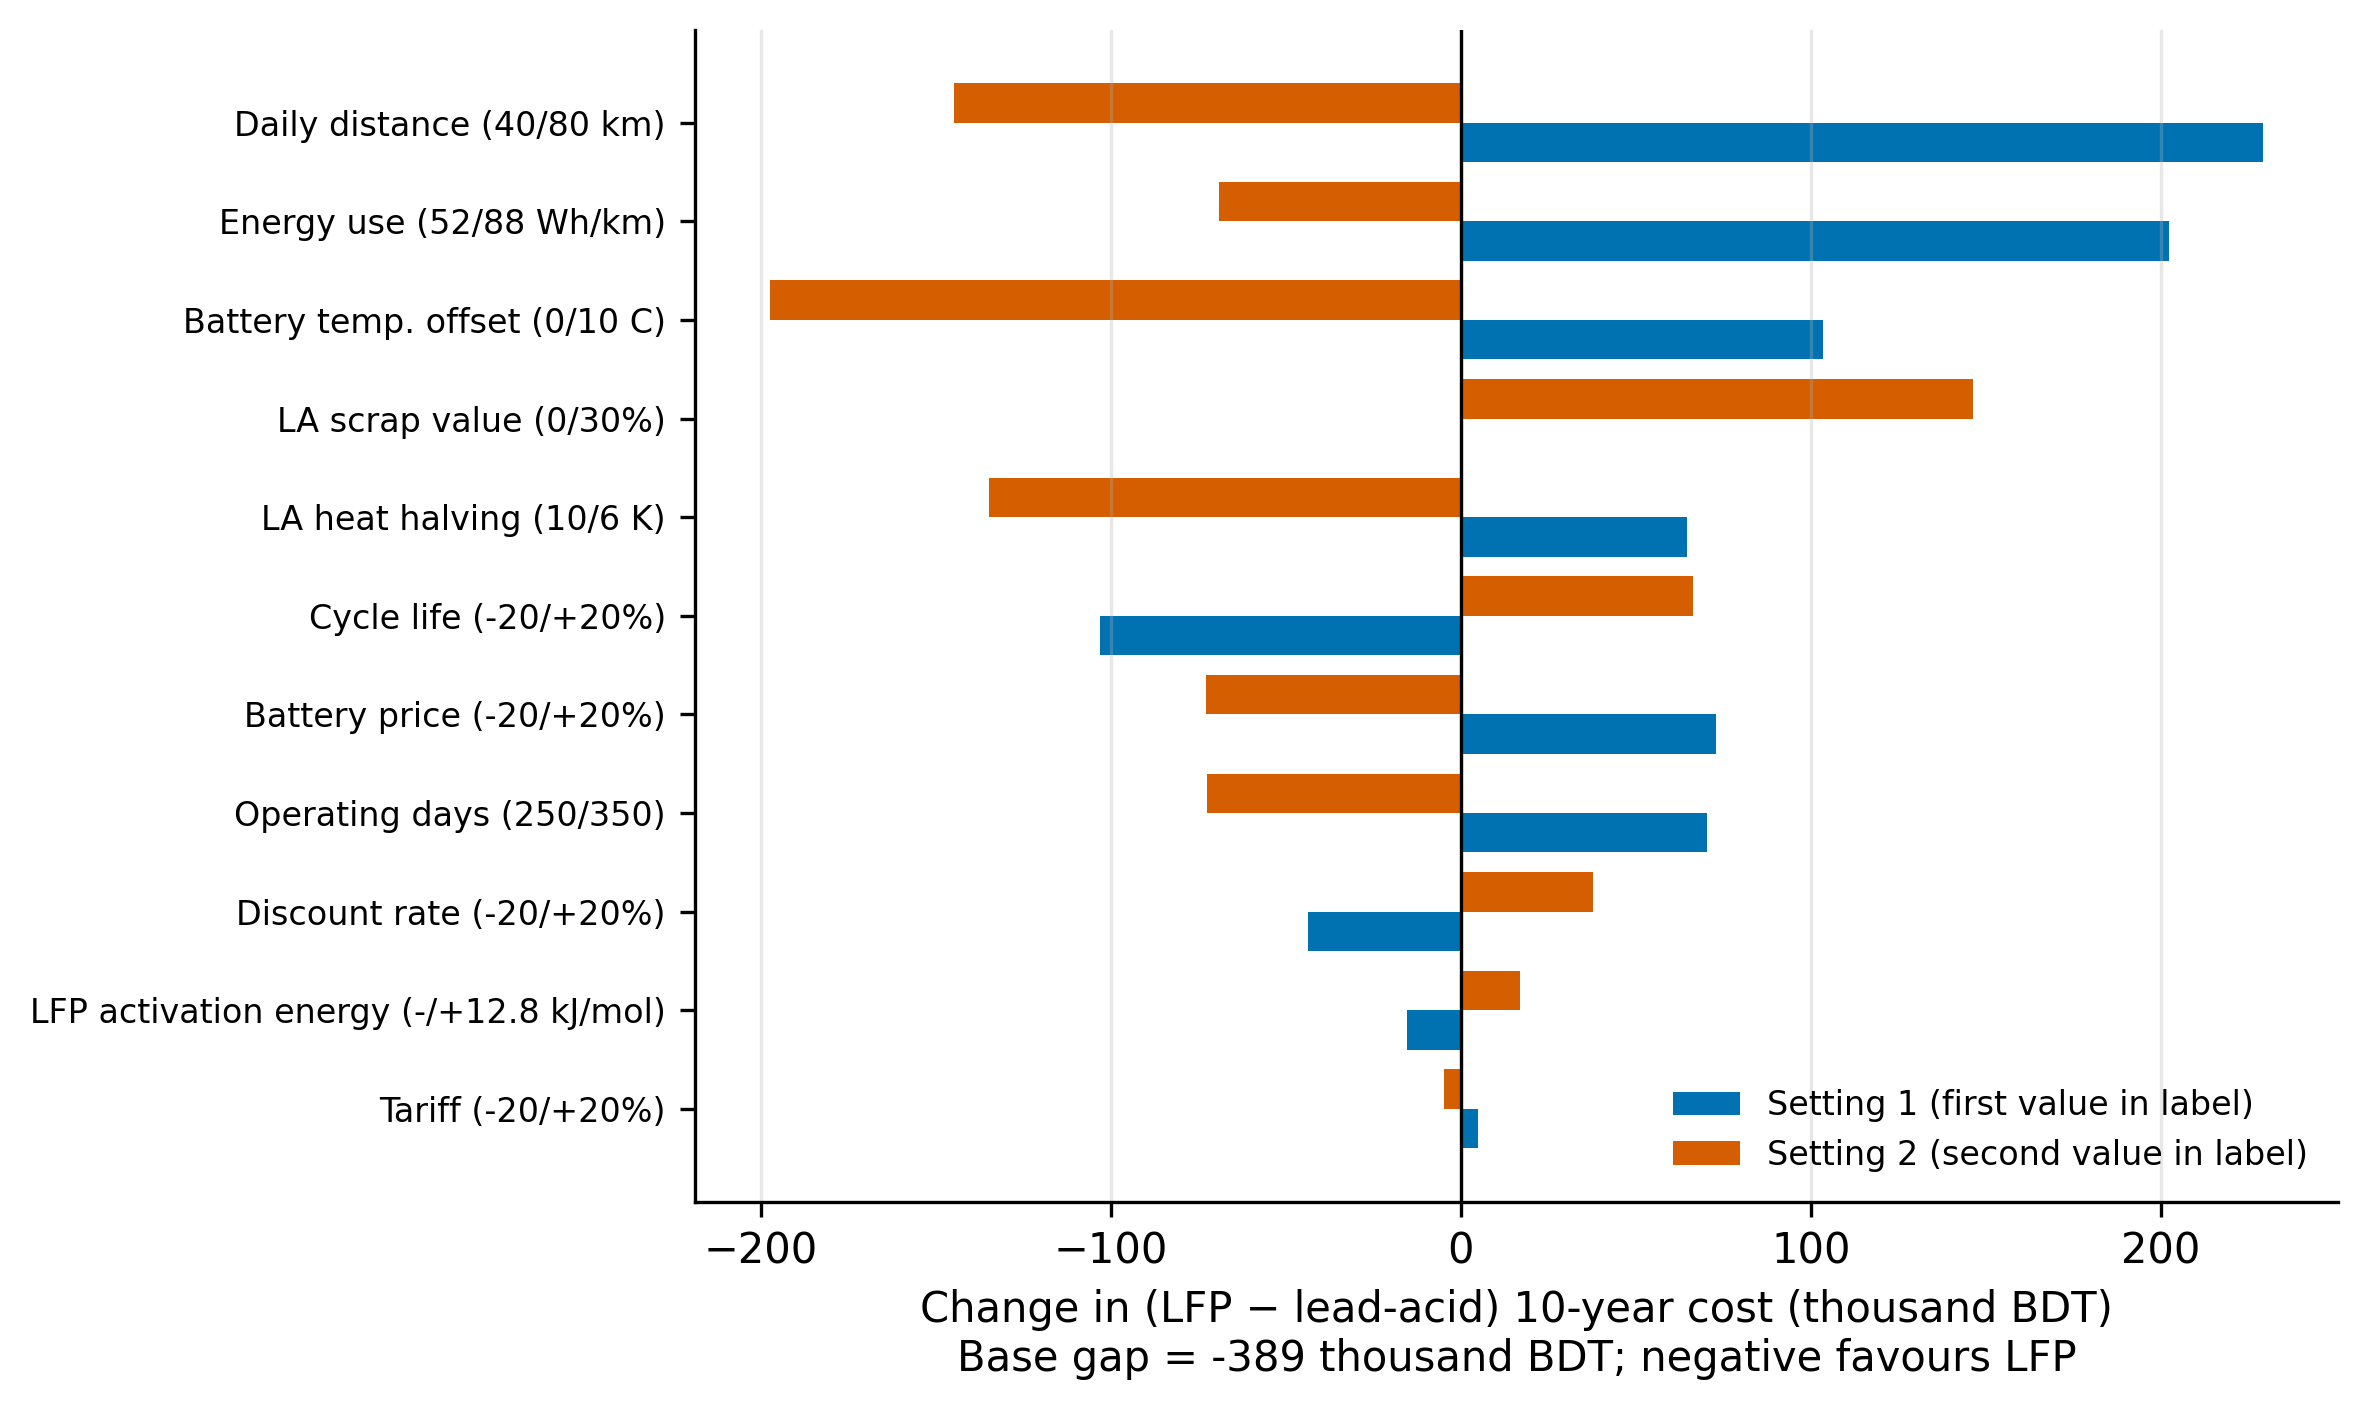
\includegraphics[width=.85\textwidth]{fig4_tornado.png}\caption{One-at-a-time sensitivity of the LFP-minus-LA 10-year cost gap at Chuadanga (base gap $-$\gapBase\ BDT). Negative values favour LFP.}\label{fig:tornado}\end{figure}
\paragraph{When does LFP stop being cheaper?} We combined the settings most unfavourable to LFP: 40~km per day, no battery heating, LA scrap value 30\% of price, LA halving every 10~K, and an LFP price 20\% above the model value. LFP is still cheaper by BDT \jointGap{}. If the LFP price is 50\% higher in that same case, LA becomes cheaper by BDT \jointGapHigh. LFP's cost advantage is therefore robust to any single assumption but not to a combination of several, and the LA scrap value is the most important missing datum (\cref{tab:scen} and the tornado: a 30\% scrap value cuts the gap by BDT \scrapThirty).

\subsection{Validation}
V1 passed (24 months per site, no gaps). V2 passed: 79.7~Wh/km lies inside the 52--88~Wh/km spanned by the published values. V3 (\cref{fig:valid}): LFP life (\lifeLFP~mo) lies at the upper edge of the 60--84 reported; LA life (\lifeLA~mo) is \vLApct\% above the 8--12 months field range; NMC life (\lifeNMC~mo) is \vNMCpct\% above 36--48. V4: modelled lead-acid grid energy (\vEgrid~kWh per bike-day) is \vCleanPct\% below the CLEAN-implied \vClean~kWh, a gap that only field metering can resolve (the CLEAN figure may include other vehicle types and charging losses). V5 is the Simulink cross-check described in the Methodology. The model is therefore plausible against the published ranges but is \emph{not} validated against operator records.
\begin{figure}[t]\centering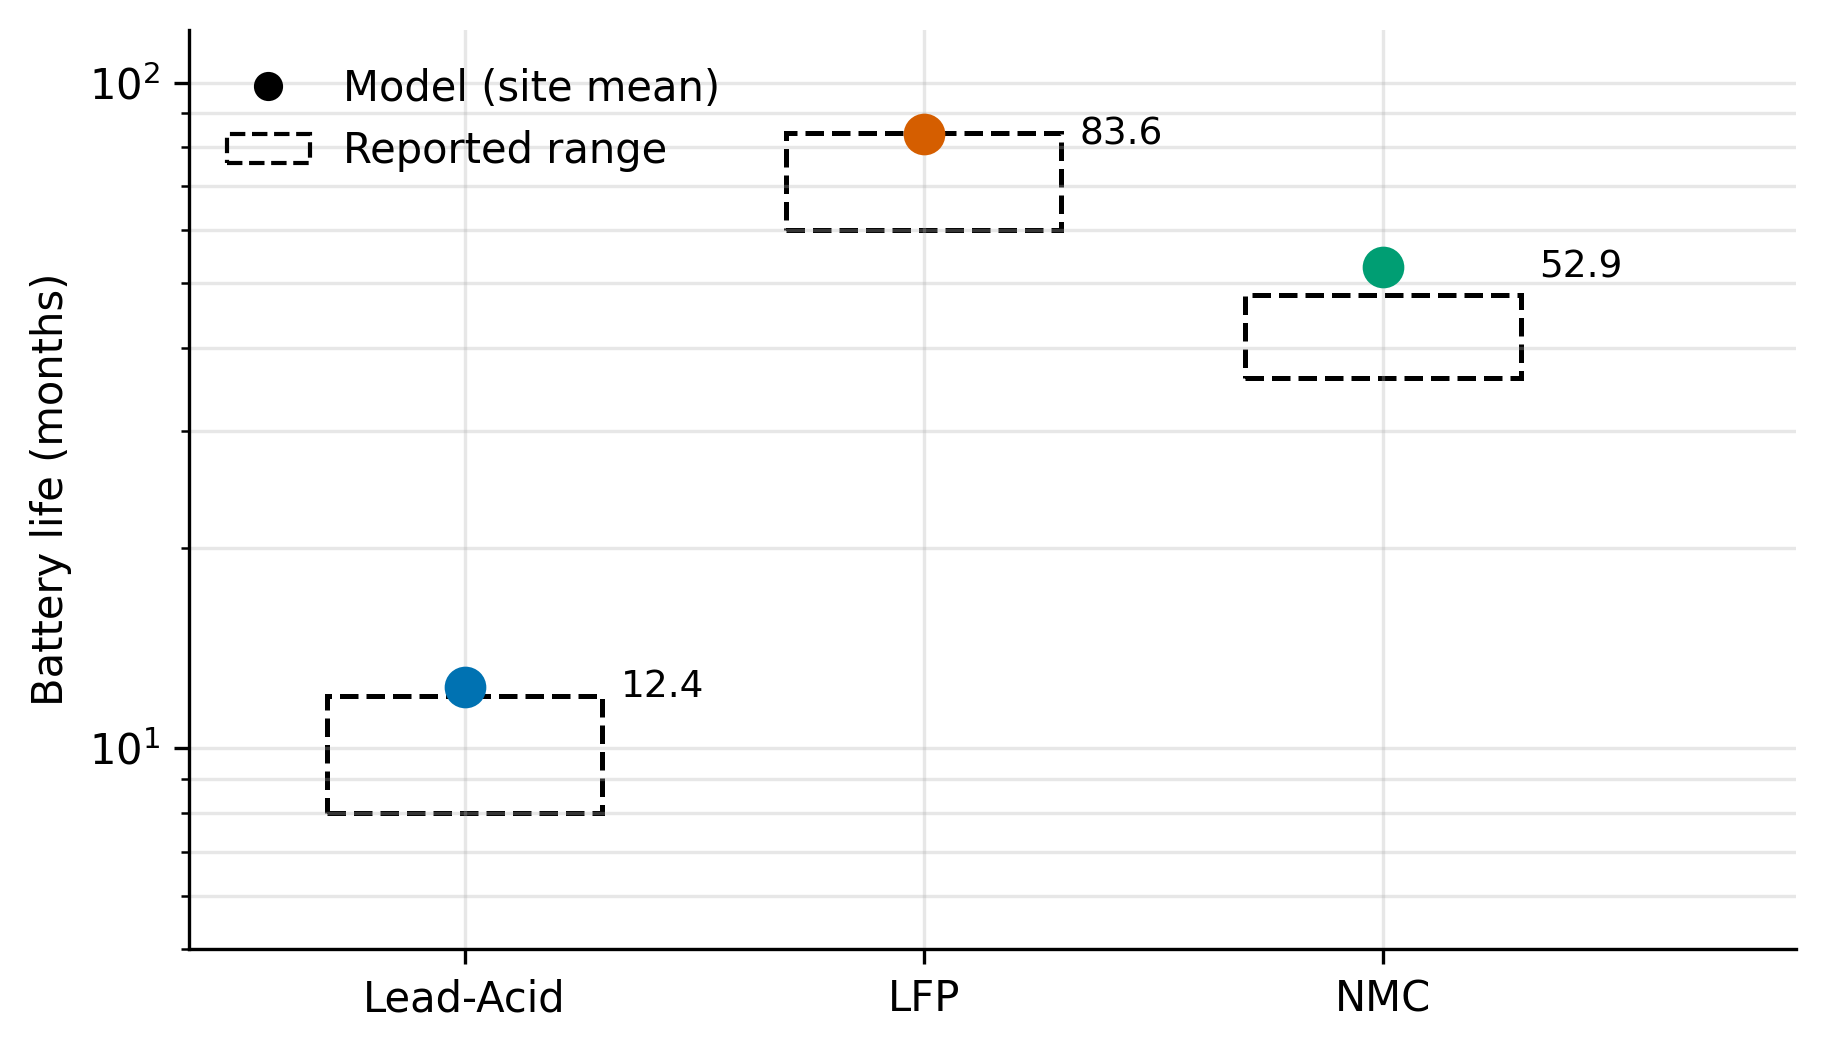
\includegraphics[width=.6\textwidth]{fig_valid.png}\caption{Modelled battery life (site mean) against reported ranges (dashed boxes; logarithmic axis).}\label{fig:valid}\end{figure}

\subsection{Carbon footprint}
\begin{table}[t]
\centering\small
\caption{Carbon budget per bike per year (site-averaged; grid factor 0.62~tCO$_2$/MWh; manufacture+end-of-life factors per kWh of pack capacity: 40 (lead-acid), 50 (LFP), 78.4 (NMC) kg\,CO$_2$e).}
\label{tab:co2bike}
\begin{tabular}{lrrrr}
\toprule
Battery & Packs/yr & Operation & Manufacture+EOL & Total \\
 & (--) & (kg CO$_2$e) & (kg CO$_2$e) & (kg CO$_2$e) \\
\midrule
Lead-acid & 0.97 & 1508 & 350 & 1858 \\
LFP & 0.14 & 1279 & 55 & 1334 \\
NMC & 0.23 & 1308 & 138 & 1447 \\
\bottomrule
\end{tabular}
\end{table}

A lead-acid easy-bike causes about \perbikeLA{}~kg\,CO$_2$e per year, an LFP bike \perbikeLFP{} and an NMC bike \perbikeNMC{} (\cref{tab:co2bike,fig:co2}). Switching one bike to LFP saves \saveLFPbike{}~kg\,CO$_2$e per year, \saveLFPop{} from lower electricity use and \saveLFPemb{} from fewer manufactured packs (\packsLA{} LA packs against \packsLFP{} LFP packs per year). For 1.4~M bikes this is \fleetLFPa{}~Mt\,CO$_2$e per year, or \fleetLFPb{}~Mt for 3~M bikes (\cref{tab:co2fleet}). The independent CLEAN-based estimate, electricity only, gives \cleanGWh{}~GWh and \cleanMt{}~Mt\,CO$_2$ per year. The per-bike saving stays between \sensMin{} and \sensMax{}~kg per year for LFP manufacturing between 50 and 110~kg\,CO$_2$e/kWh and grid factors of 0.55--0.70 (\cref{fig:co2sens}).
\begin{figure}[t]\centering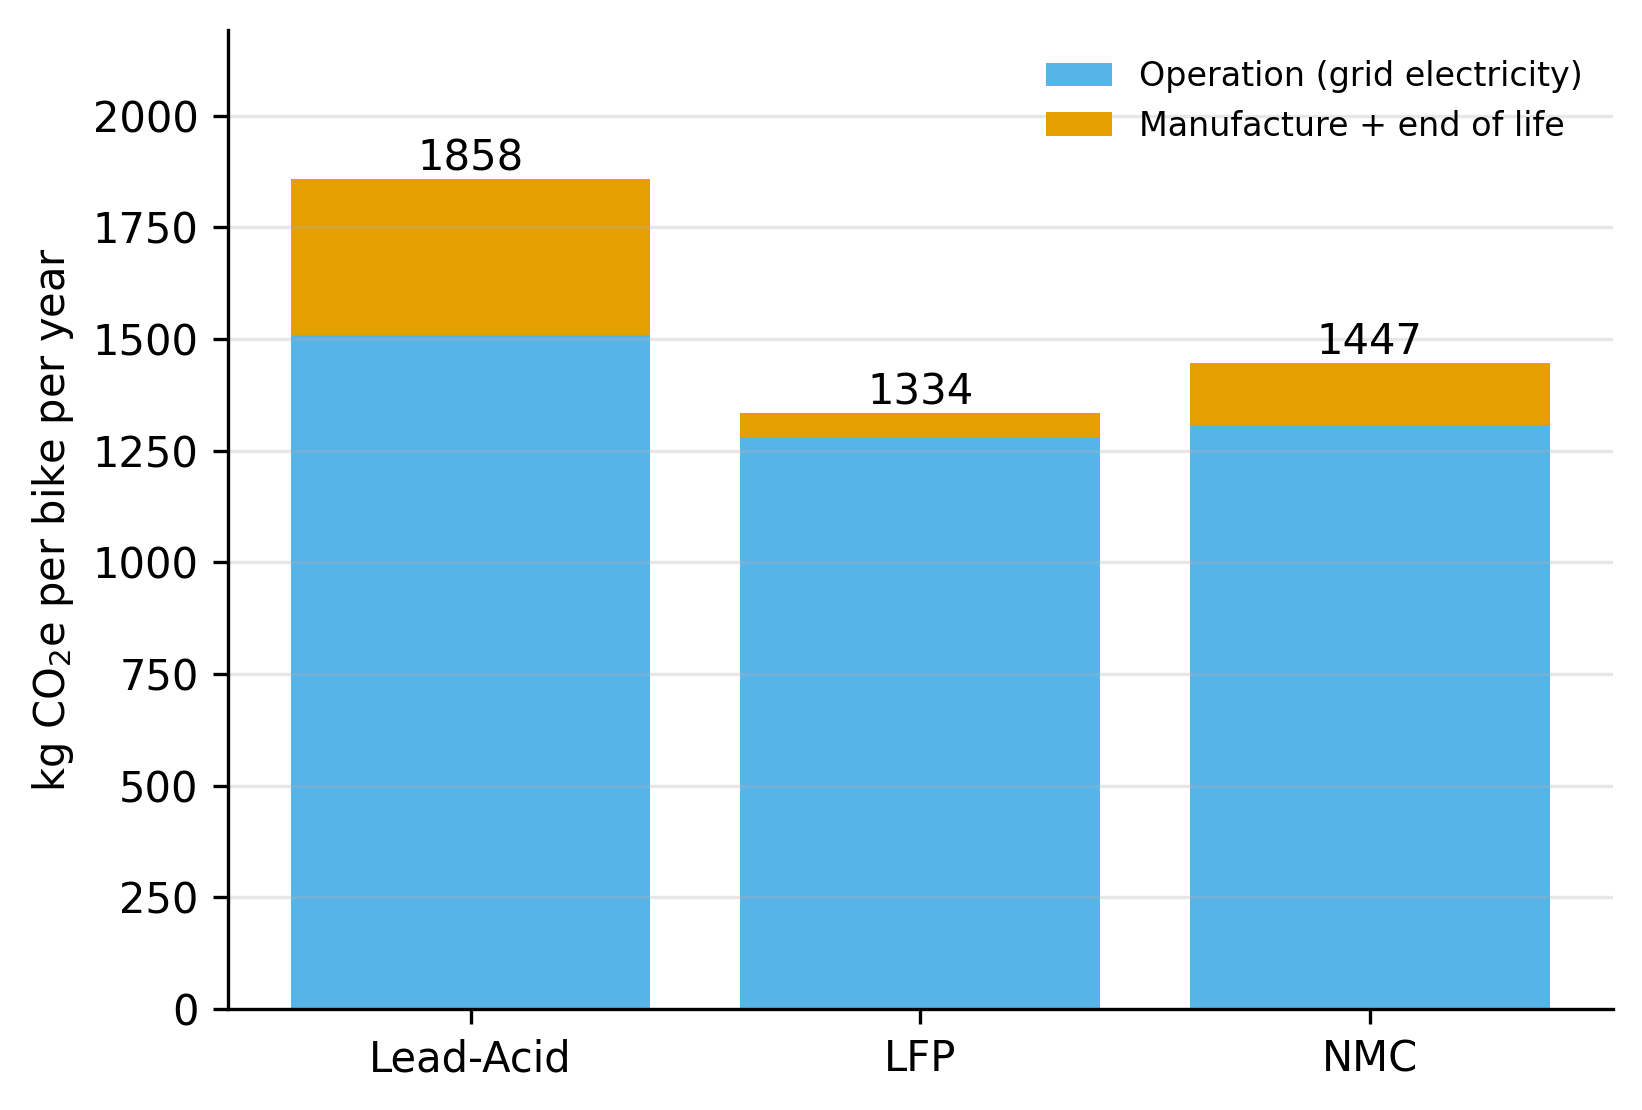
\includegraphics[width=.62\textwidth]{fig5_co2_bike.png}\caption{Annual carbon footprint per bike, split into operation and manufacture+end-of-life.}\label{fig:co2}\end{figure}
\begin{table}[t]
\centering\small
\caption{Fleet-level annual CO$_2$e under two fleet-size scenarios; savings are lead-acid minus the alternative if the \emph{entire} fleet switched.}
\label{tab:co2fleet}
\begin{tabular}{lrr}
\toprule
 & 1.4 M bikes \citep{clean2024} & 3.0 M bikes (lower bound of 3--4 M \citep{pureearth_smep}) \\
 & (Mt CO$_2$e/yr) & (Mt CO$_2$e/yr) \\
\midrule
Lead-acid fleet (baseline) & 2.60 & 5.57 \\
Saving, all LFP (operation) & 0.32 & 0.69 \\
Saving, all LFP (manufacture+EOL) & 0.41 & 0.88 \\
\textbf{Saving, all LFP (total)} & \textbf{0.73} & \textbf{1.57} \\
Saving, all NMC (total) & 0.58 & 1.23 \\
\bottomrule
\end{tabular}
\end{table}

\begin{figure}[t]\centering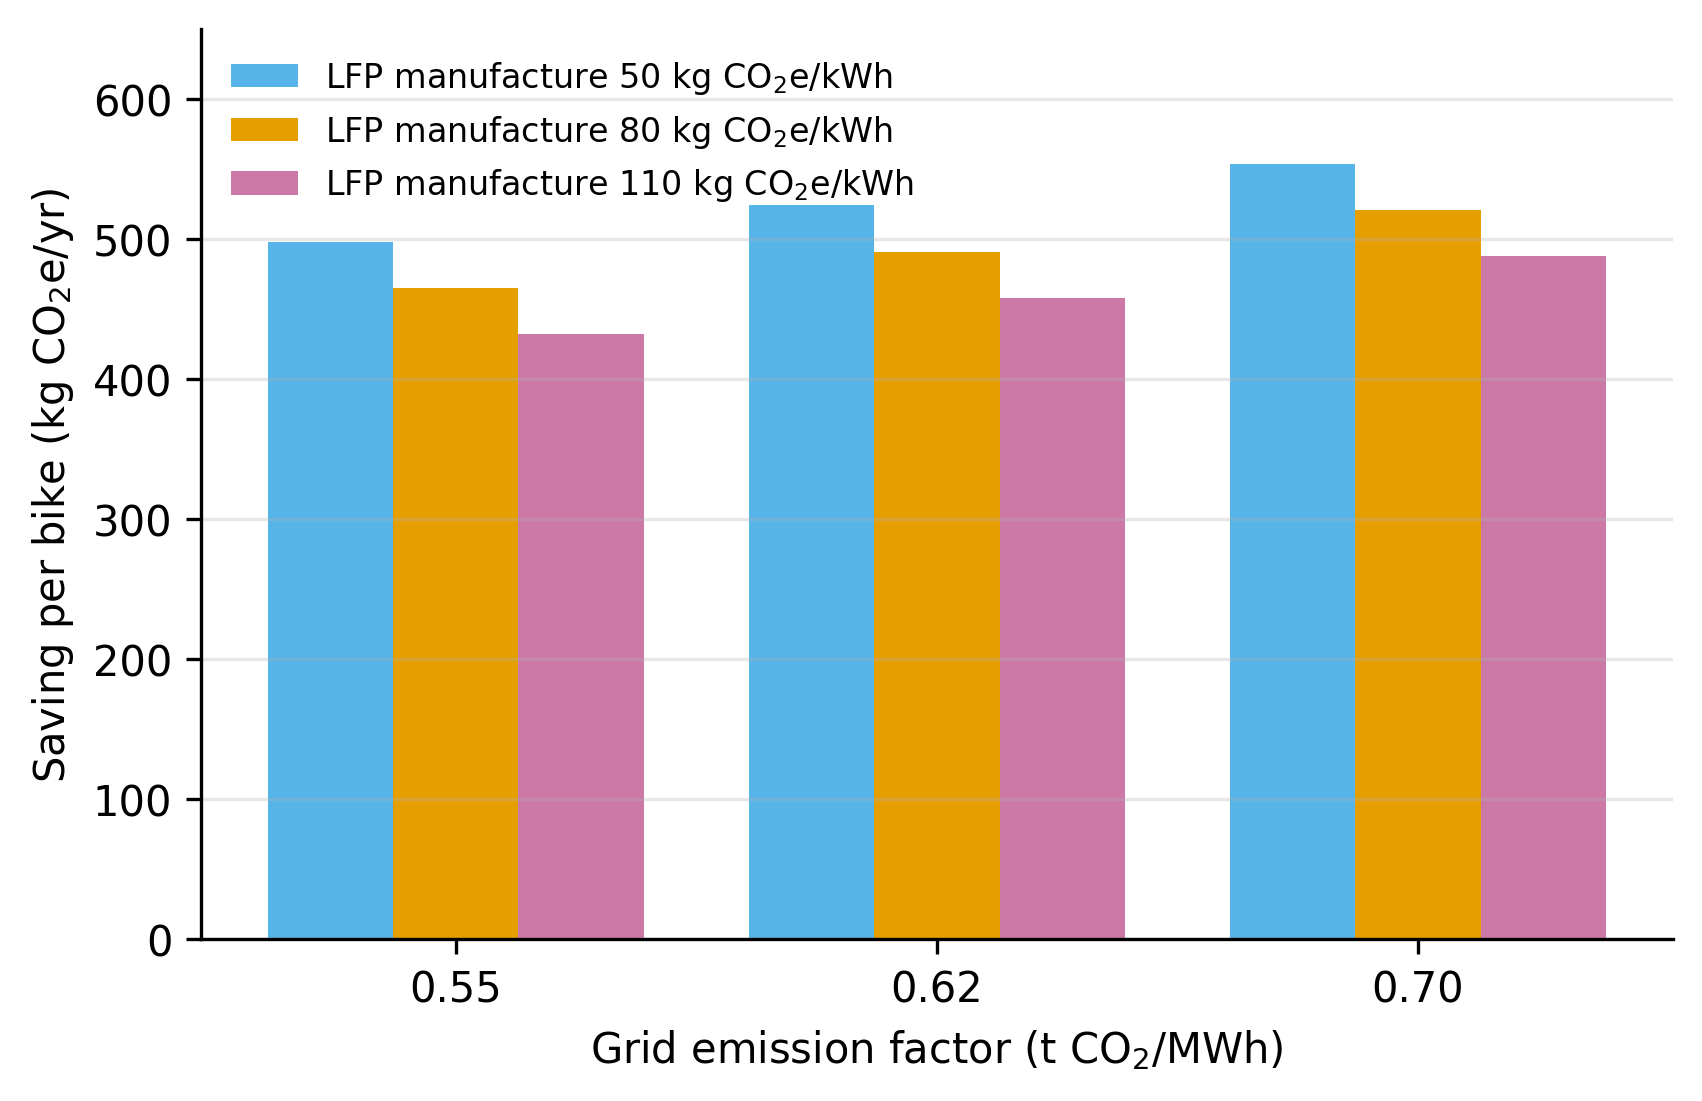
\includegraphics[width=.62\textwidth]{fig7_co2_sensitivity.png}\caption{Per-bike saving from LFP versus lead-acid for three LFP manufacturing footprints and three grid emission factors.}\label{fig:co2sens}\end{figure}

\subsection{Lead flow and policy scenarios}
\begin{table}[t]
\centering\small
\caption{Lead throughput of the lead-acid fleet (kt Pb per year through replacement and recycling). 125~kg is the figure published by Pure Earth \citep{pureearth_smep}; 60 and 90~kg are scenarios (battery mass $\times$ lead share).}
\label{tab:lead}
\begin{tabular}{lrr}
\toprule
Lead per pack & 1.4 M bikes & 3.0 M bikes \\
\midrule
60 kg & 82 & 175 \\
90 kg & 122 & 262 \\
125 kg & 170 & 364 \\
\bottomrule
\end{tabular}
\end{table}

\begin{table}[t]
\centering\small
\caption{Policy scenarios for a 1.4~M-bike fleet: share moved from lead-acid to LFP. Lead flow assumes 90~kg Pb per pack (60--125~kg, \cref{tab:lead}); savings are 10-year NPV to operators.}
\label{tab:policy}
\begin{tabular}{lrrrr}
\toprule
Scenario & LFP share & CO$_2$e saved & Pb cycled & Operator saving \\
 & (\%) & (Mt/yr) & (kt Pb/yr) & ($10^9$ BDT) \\
\midrule
S0 Business as usual & 0 & 0.00 & 122 & 0 \\
S1 Early adoption & 25 & 0.18 & 92 & 135 \\
S2 Targeted policy & 50 & 0.37 & 61 & 270 \\
S3 Full transition & 100 & 0.73 & 0 & 539 \\
\bottomrule
\end{tabular}
\end{table}

The lead-acid fleet cycles \leadLow--\leadHigh{}~kt of lead per year at 1.4~M bikes (\cref{tab:lead}); the upper value is close to the 167~kt reported by Pure Earth for the whole electric three-wheeler sector \citep{pureearth_smep}. Converted bikes need replacement so rarely that their lead flow in the model falls to zero. A 50\% conversion saves \polHalfCO{}~Mt\,CO$_2$e per year and BDT \polHalfSav{} billion for operators over ten years, and full conversion saves \polFullCO{}~Mt per year and BDT \polFullSav{} billion (\cref{tab:policy,fig:policy}).
\begin{figure}[t]\centering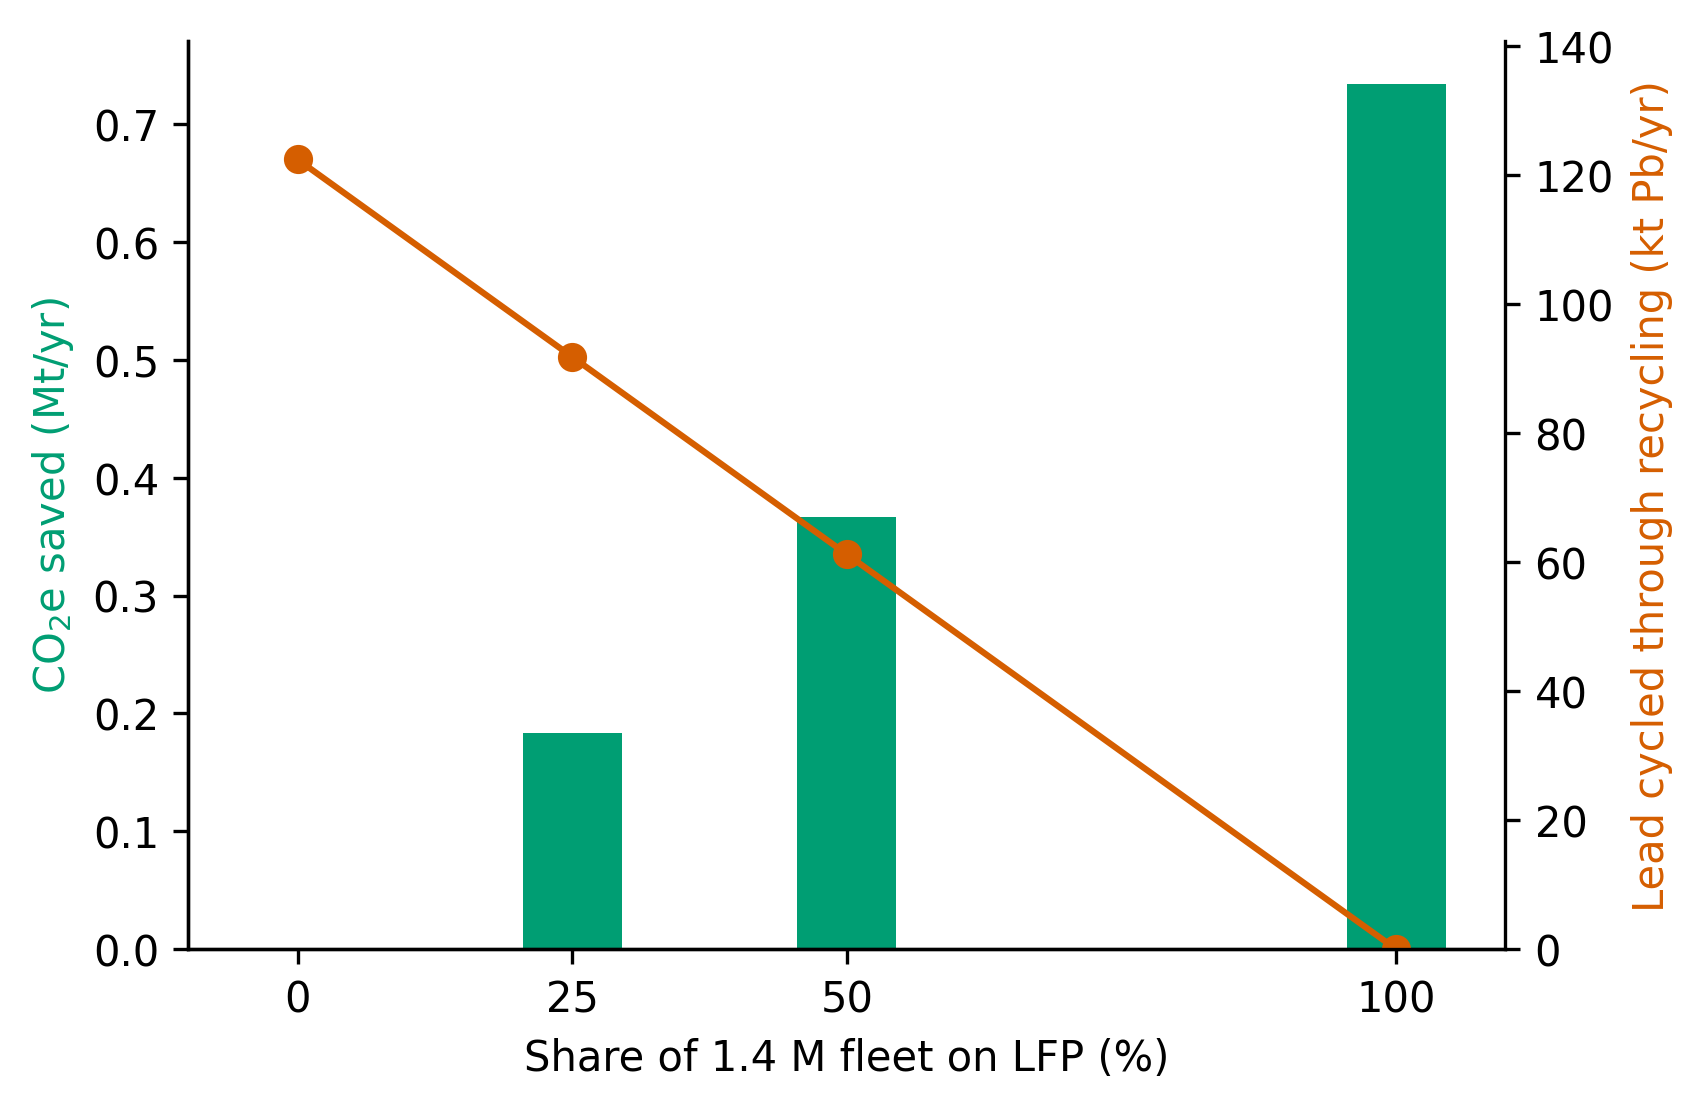
\includegraphics[width=.62\textwidth]{fig6_policy.png}\caption{Policy scenarios: CO$_2$e saved and lead cycled through recycling versus the share of the fleet on LFP.}\label{fig:policy}\end{figure}
